\documentclass{standalone}
\usepackage{pgfplots}
\pgfplotsset{compat=newest}
\usepgfplotslibrary{patchplots}
\begin{document}
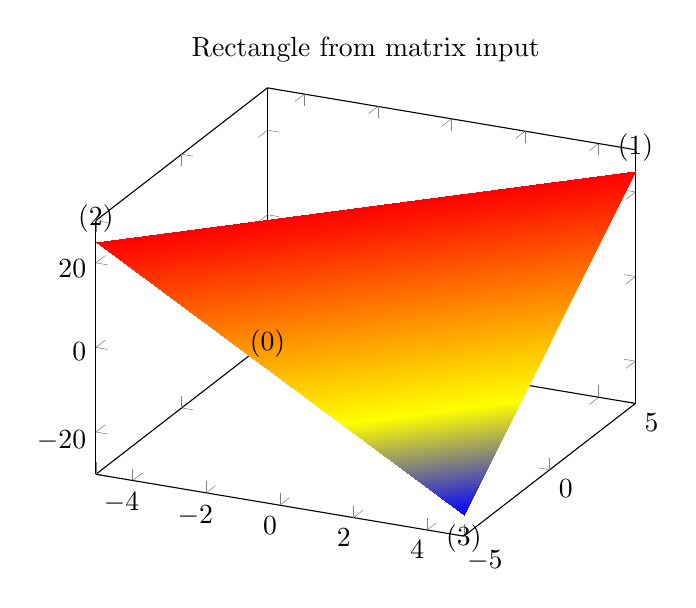
\begin{tikzpicture}
\begin{axis}[nodes near coords={(\coordindex)},
	title=Rectangle from matrix input]
% note that surf implies 'patch type=rectangle'
\addplot3[surf,shader=interp,samples=2,
	patch type=rectangle] 
	{x*y};
\end{axis}
\end{tikzpicture}
\end{document}
